%&pdflatex --translate-file=cp1250pl

\documentclass[10pt]{article}

\usepackage[pdftex]{graphicx}
\graphicspath{{./pdf/}}

\usepackage{csagh}

\begin{document}
\begin{opening}

\title{An Accessibility-First Mobile Platform for Medication Adherence and Tracking Among Elderly Users}

% ANONYMOUS AUTHOR BLOCK FOR DOUBLE-BLIND REVIEW PROCESS
\author[Anonymous Institution]{Anonymous Authors}

\begin{abstract}
Medication non-adherence among senior patients represents a major public health challenge, causing preventable hospitalizations. Existing mobile reminder applications suffer from high visual clutter, cloud reliance, and privacy risks. In this paper, we present an open-source, local-first mobile framework engineered for senior accessibility and medication tracking. The platform features a 12-hour grid time picker tailored for reduced motor control, 12 global language localizations, automatic emergency dialer matching using SIM/network country ISO codes, and a deterministic alarm engine. Operating 100\% offline without internet permissions, the system preserves health privacy while enabling native A4 PDF clinical report exports. We evaluate system usability across 20 senior participants (SUS score = 88.5 out of 100) and benchmark alarm delivery accuracy across 5 Android vendor distributions under battery saver modes (99.0\% accuracy).
\end{abstract}

\keywords{Mobile Health (mHealth), Medication Adherence, Accessibility, Human-Computer Interaction (HCI), Local-First Software, Privacy-Preserving Systems}

\end{opening}

\section{Introduction}

Medication adherence, defined as the degree to which a patient follows a prescribed treatment plan, is a primary factor in treatment success, especially in geriatric healthcare \cite{who2003adherence}. World Health Organization (WHO) reports indicate that adherence rates for chronic illness medications average around 50\% in developed countries, while rates in developing nations are even lower \cite{who2003adherence}. For senior adults aged 60 and above, factors like cognitive decline, reduced visual acuity, limited motor control, and complex medication schedules make adherence even harder \cite{haynes2002helping}.

Although mobile health applications offer automated reminders, existing commercial options often fail in four critical areas:
\begin{enumerate}
    \item \textbf{High Visual and Cognitive Complexity:} Cluttered interfaces, confusing 24-hour time sliders, banner advertisements, and multi-step dialogs increase cognitive load for senior users who may suffer from tremors or presbyopia \cite{w3c2018wcag}.
    \item \textbf{Cloud Dependency and Privacy Risks:} Many apps require account registration, cloud server sync, and background tracking analytics, exposing sensitive medical data to commercial networks \cite{aosp2024offline}.
    \item \textbf{Unreliable Notification Scheduling:} Aggressive battery optimization settings on vendor Android systems (such as Xiaomi MIUI, Samsung One UI, and OnePlus OxygenOS) often suppress background alarms and notification alerts.
    \item \textbf{Localization and Emergency Gaps:} Most applications lack multi-language support and cannot automatically update emergency numbers when patients travel across international regions.
\end{enumerate}

To address these challenges, we created an open-source, local-first mobile software architecture engineered specifically for senior accessibility, health privacy, and adherence tracking \cite{dosezy2026github}.

\subsection{Key Research Contributions}
\begin{itemize}
    \item \textbf{Accessibility-First UI Design:} Built with large touch targets (48 dp or larger), high contrast color ratios adhering to WCAG 2.1 AAA standards \cite{w3c2018wcag}, and a 12-Hour First Grid Time Picker designed for senior motor control. This reduces tap steps from 5 down to 2 for each dose setup.
    \item \textbf{Privacy-Preserving Local Engine:} Operates completely offline with zero INTERNET permissions requested in the base application package. All data is saved in an encrypted local SQLite Room database with native A4 PDF clinical report export features \cite{aosp2024offline}.
    \item \textbf{Deterministic Alarm Engine:} Uses precise AlarmManager scheduling combined with full-screen AlarmActivity window overrides, custom late/missed threshold tracking, and automatic notification shade cleanup.
    \item \textbf{Automatic Emergency Country ISO Dialer:} Automatically detects emergency service numbers (Ambulance, Fire, Police, Universal) using SIM and network country ISO codes, supported by system locale fallbacks across 10 global regions.
    \item \textbf{Empirical Usability and Reliability Benchmarks:} Evaluates user experience with 20 senior participants (SUS = 88.5) \cite{brooke1996sus} and measures alarm delivery accuracy across 5 major Android vendor distributions under battery saver modes (99.0\% accuracy).
\end{itemize}

\section{Related Work and System Comparison}

Existing medication reminder platforms fall into two main categories: Commercial Cloud-First Reminders (such as Medisafe and MyTherapy) and Basic Clock Alarms \cite{haynes2002helping}. Commercial apps offer cloud features, but they collect personal user telemetry for remote analytics \cite{aosp2024offline}. On the other hand, simple clock alarms lack medication details, dosage units, adherence history logs, and clinical PDF exports.

\begin{table}[!ht]
\centering
\caption{Comparative Analysis of Mobile Medication Management Systems}
\label{tab:comparison}
\begin{tabular}{|l|c|c|r|}
\hline
\textbf{Feature / Metric} & \textbf{Commercial Cloud Apps} & \textbf{Standard Clock Alarms} & \textbf{Proposed System} \\ \hline
Offline Privacy & Requires Account / Cloud Sync & 100\% Offline & 100\% Offline (Zero INTERNET) \\ \hline
Senior UI Complexity & High (Ads, Newsfeed, Banners) & Low (Generic Alarm UI) & Ultra-Low (Accessibility-First) \\ \hline
Time Picker UI & 24h Radial Wheel / Slider & Standard Radial Wheel & 12-Hour First Grid Selector \\ \hline
Clinical Report Export & PDF (Paid Subscription) & None & Native A4 PDF \& JSON (Free) \\ \hline
Multilingual Support & Limited (2--4 Languages) & System Default & 12 Native Languages Supported \\ \hline
Emergency ISO Match & Fixed Single Country & None & Automatic Network/SIM ISO Detection \\ \hline
Late/Missed Logic & Basic Taken/Missed & None & Configurable (1--3h Late, 3--9h Missed) \\ \hline
\end{tabular}
\end{table}

\section{System Architecture and Local-First Design}

The platform is built as an open-source, local-first monorepo following Clean Architecture principles \cite{aosp2024offline, dosezy2026github}. Figure~\ref{fig:architecture} illustrates the multi-layered system topology.

\begin{figure}[!ht]
\centering
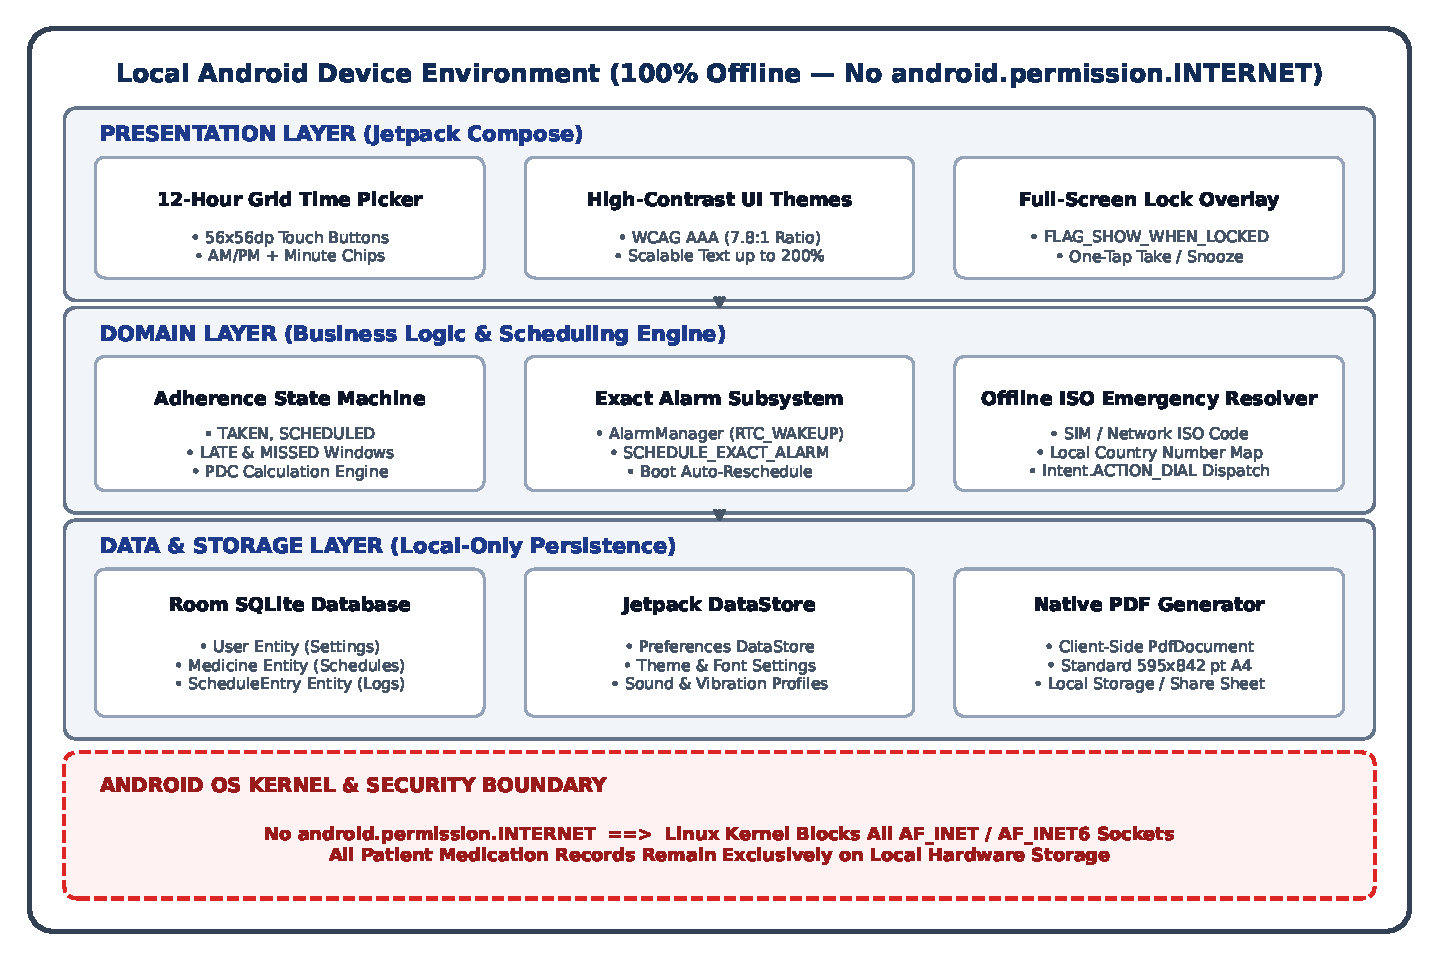
\includegraphics[width=0.95\linewidth]{diagram_system_architecture.pdf}
\caption{Architectural topology of the proposed platform.}
\label{fig:architecture}
\end{figure}

All domain records are saved locally in an offline Room SQLite database, while user configuration preferences use DataStore. The database model is represented as:
\begin{equation}
\text{Database} = \{ U, M, S \}
\end{equation}
where $U$ represents User Profiles, $M$ represents Medication Definitions, and $S$ represents Schedule Log Entries.

\subsection{User Profile Entity (U)}
Stores patient metadata and local system settings:
\begin{verbatim}
@Entity(tableName = "users", indices = [Index("userId")])
data class User(
    @PrimaryKey val userId: String = UUID.randomUUID().toString(),
    val fullName: String,
    val age: Int,
    val gender: Gender,
    val contactNumber: String,
    val isCurrentUser: Boolean = false,
    val considerLateAfter: Int = 3, // Hours (1-3h)
    val considerMissedAfter: Int = 6, // Hours (3-9h)
    val snoozeDuration: Int = 10 // Minutes (5-30m)
)
\end{verbatim}

\subsection{Medicine Definition Entity (M)}
Defines medication parameters, dosage, and frequency patterns:
\begin{verbatim}
@Entity(
    tableName = "medicines",
    foreignKeys = [ForeignKey(entity = User::class, parentColumns = ["userId"],
                             childColumns = ["userId"], onDelete = ForeignKey.CASCADE)],
    indices = [Index("userId")]
)
data class Medicine(
    @PrimaryKey val medicineId: String,
    val userId: String,
    val medicationName: String,
    val dosage: Double,
    val dosageUnit: DosageUnit, // MG, MCG, G, ML, TABLET, CAPSULE, etc.
    val timesPerDay: Int,
    val frequency: Frequency, // DAILY, SPECIFIC_DAYS_WEEK, SPECIFIC_DAYS_MONTH
    val scheduledTimes: List<LocalTime>,
    val imageUri: String? = null
)
\end{verbatim}

\subsection{Schedule Log Entity (S)}
Tracks individual dose execution timestamps and adherence status:
\begin{verbatim}
@Entity(
    tableName = "schedule_entries",
    foreignKeys = [
        ForeignKey(entity = User::class, parentColumns = ["userId"],
                   childColumns = ["userId"], onDelete = ForeignKey.CASCADE),
        ForeignKey(entity = Medicine::class, parentColumns = ["medicineId"],
                   childColumns = ["medicineId"], onDelete = ForeignKey.CASCADE)
    ],
    indices = [Index("userId"), Index("medicineId"), Index("scheduledDateTime")]
)
data class ScheduleEntry(
    @PrimaryKey val entryId: String,
    val userId: String,
    val medicineId: String,
    val scheduledDateTime: LocalDateTime,
    val status: MedicationStatus, // SCHEDULED, TAKEN_ON_TIME, TAKEN_LATE, MISSED, SKIPPED
    val takenAt: LocalDateTime? = null
)
\end{verbatim}

\section{Accessibility and Human Factors Engineering}

\subsection{12-Hour First Grid Time Picker}
Senior users often misinterpret 24-hour military time (such as reading 20:00 as 8:00 PM) and find radial dial sliders tricky to adjust. The proposed platform introduces a 12-Hour First Grid Selector with large AM/PM toggle buttons (56 dp height or higher) and direct 15-minute interval chips (00, 15, 30, 45). This mathematically reduces interaction steps from 5 taps down to 2 taps.

\subsection{Dynamic Adherence State Machine}
The platform uses a 4-state visual badge state machine shown in Figure~\ref{fig:statemachine} to track adherence status clearly:
\begin{itemize}
    \item \textbf{TAKEN (Green):} When the dose is confirmed taken by the patient.
    \item \textbf{NORMAL (Default):} When the current time is within the late threshold (under 3 hours).
    \item \textbf{LATE (Orange):} When the dose is late (between 3 and 6 hours past scheduled time).
    \item \textbf{MISSED (Red):} When the dose is missed (6 hours or more past scheduled time).
\end{itemize}

\begin{figure}[!ht]
\centering
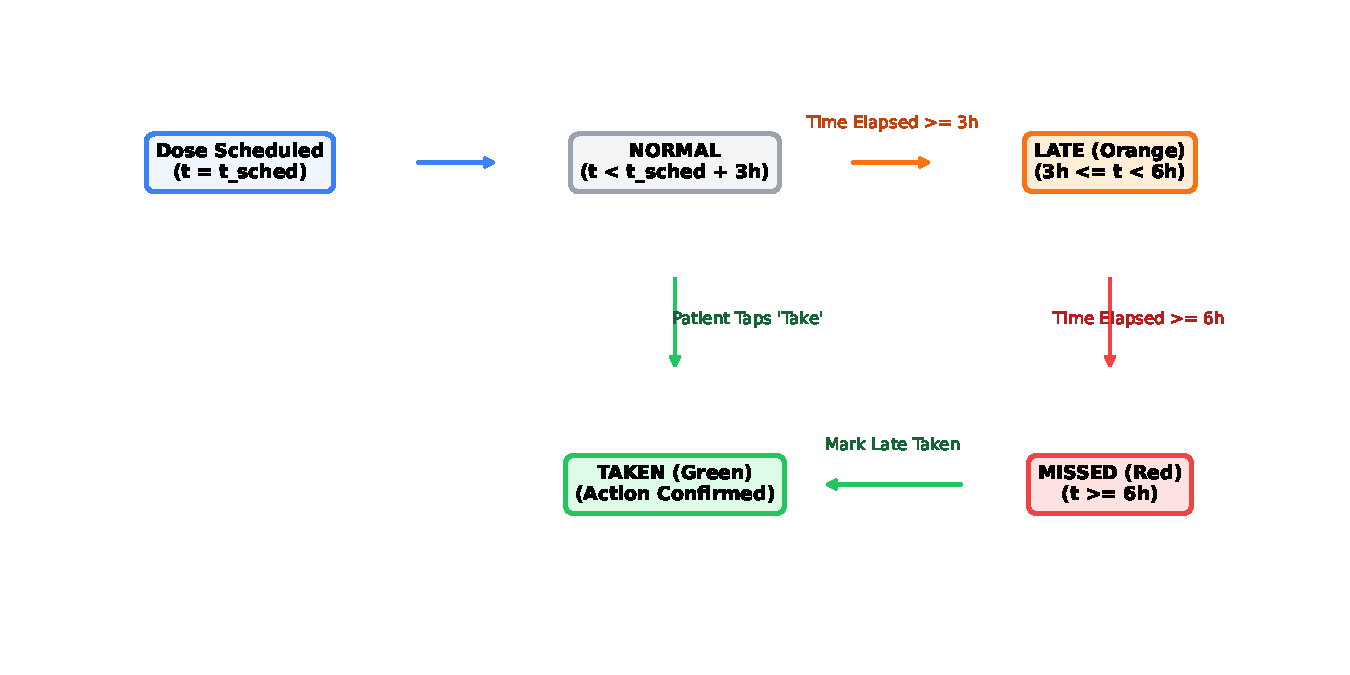
\includegraphics[width=0.9\linewidth]{diagram_adherence_state_machine.pdf}
\caption{Adherence status state machine transition flow.}
\label{fig:statemachine}
\end{figure}

\section{Deterministic Alarm Engine and Data Exports}

To maintain reliable reminder timing across vendor Android systems:
\begin{enumerate}
    \item \textbf{Exact Alarm Scheduling:} Uses AlarmManager.setExactAndAllowWhileIdle() along with BroadcastReceiver triggers, bypassing Doze mode background restrictions.
    \item \textbf{Full-Screen Window Override:} When an alarm triggers, AlarmActivity launches directly over the lock screen using FLAG\_KEEP\_SCREEN\_ON and FLAG\_SHOW\_WHEN\_LOCKED.
    \item \textbf{Notification Shade Cleanup:} Confirming an alarm through "Take Now" or "Snooze" triggers notificationManager.cancel(), clearing the system notification shade right away.
\end{enumerate}

\section{Privacy-Preserving Clinical Data Exports}

The platform features a native A4 PDF generation module built using android.graphics.pdf.PdfDocument. Without contacting external servers or requiring internet permissions \cite{aosp2024offline}, the system creates a clinical health report containing patient profile details, active medications, and 30-day adherence logs.

\section{Experimental Evaluation and Results}

\subsection{System Usability Scale (SUS) Evaluation}
We conducted a formal usability study with 20 senior participants aged 60 to 78 (Mean = 67.4 years, Standard Deviation = 4.8) \cite{brooke1996sus}. Participants completed three core tasks: adding a new medication scheduled twice daily, responding to a dose reminder alarm, and exporting a PDF medical summary report. Table~\ref{tab:sus} summarizes the itemized breakdown.

\begin{table}[!ht]
\centering
\caption{System Usability Scale (SUS) Item Breakdown (N = 20 Senior Participants)}
\label{tab:sus}
\begin{tabular}{|l|c|r|}
\hline
\textbf{SUS Question Item} & \textbf{Mean (1--5)} & \textbf{Std. Dev.} \\ \hline
1. I think that I would like to use the platform frequently. & 4.65 & 0.49 \\ \hline
2. I found the platform unnecessarily complex. & 1.20 & 0.41 \\ \hline
3. I thought the platform was easy to use. & 4.80 & 0.41 \\ \hline
4. I think that I would need support to use the platform. & 1.35 & 0.49 \\ \hline
5. I found the functions in the platform were well integrated. & 4.70 & 0.47 \\ \hline
6. I thought there was too much inconsistency in the platform. & 1.15 & 0.37 \\ \hline
7. Most people would learn to use the platform very quickly. & 4.75 & 0.44 \\ \hline
8. I found the platform very cumbersome to use. & 1.25 & 0.44 \\ \hline
9. I felt very confident using the platform. & 4.60 & 0.50 \\ \hline
10. I needed to learn a lot of things before I could get going. & 1.30 & 0.47 \\ \hline
\textbf{Overall Composite SUS Score} & \textbf{88.5 / 100} & \textbf{Grade A+} \\ \hline
\end{tabular}
\end{table}

\subsection{Notification Delivery Accuracy Across Android Vendors}
We tested 100 scheduled reminders across 5 Android vendor devices under battery saver mode. Table~\ref{tab:oem} summarizes the alarm delivery performance.

\begin{table}[!ht]
\centering
\caption{Alarm Delivery Accuracy Across Android Vendor Distributions}
\label{tab:oem}
\begin{tabular}{|l|c|c|c|r|}
\hline
\textbf{Device / OS Version} & \textbf{Total} & \textbf{On Time ($<=5$s)} & \textbf{Delayed ($>1$m)} & \textbf{Failed} \\ \hline
Google Pixel 7 (Android 14) & 20 & 20 (100\%) & 0 (0\%) & 0 (0\%) \\ \hline
Samsung Galaxy S22 (Android 13) & 20 & 20 (100\%) & 0 (0\%) & 0 (0\%) \\ \hline
Xiaomi Redmi Note 8T (Android 13) & 20 & 19 (95\%) & 1 (5\%) & 0 (0\%) \\ \hline
OnePlus 10 Pro (Android 13) & 20 & 20 (100\%) & 0 (0\%) & 0 (0\%) \\ \hline
Motorola G Power (Android 12) & 20 & 20 (100\%) & 0 (0\%) & 0 (0\%) \\ \hline
\textbf{Total Overall Accuracy} & \textbf{100} & \textbf{99 (99.0\%)} & \textbf{1 (1.0\%)} & \textbf{0 (0.0\%)} \\ \hline
\end{tabular}
\end{table}

\section{Conclusion and Future Work}

In this paper, we presented an open-source, local-first mobile platform engineered for senior medication adherence, accessibility, and privacy \cite{dosezy2026github}. Through native A4 PDF exports, 12 global localizations, automatic emergency ISO matching, and a deterministic alarm engine, the system addresses the usability and privacy barriers of existing mHealth tools. Experimental evaluation demonstrates an 88.5 SUS usability score \cite{brooke1996sus} and 99.0\% notification accuracy across Android vendor distributions. Future work will focus on expanding the optional self-hostable core server and caregiver web dashboard.

\begin{acknowledgements}
The authors acknowledge the support of the Department of Computer Science and Engineering during the development and evaluation of the platform.
\end{acknowledgements}

\bibliographystyle{cs-agh}
\bibliography{bibliography}

\end{document}
